\subsubsection{Rancangan Detail Komponen Log Management}
\label{subsubsection:detail-data-log-management}

Komponen \textit{logging} dan \textit{tracing} bertanggung jawab untuk mencatat dan melacak aktivitas sistem. Komponen ini akan mengumpulkan data dari berbagai komponen lain dalam sistem, termasuk informasi tentang permintaan yang diterima, respons yang dikirim, dan status sistem secara keseluruhan. Ilustrasi struktur komponen \textit{log management} dapat dilihat pada Gambar \ref{fig:log-management-structure}.

\begin{figure}[ht]
    \centering
    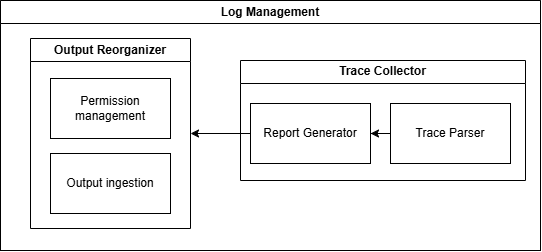
\includegraphics[width=0.55\textwidth]{resources/chapter-3/log-management-architecture.png}
    \caption{Struktur Komponen Log Management}
    \label{fig:log-management-structure}
\end{figure}

Tugas komponen \textit{log management} relatif sederhana, yaitu mengumpulkan data dari hasil \textit{log} yang dihasilkan \textit{node} lalu membangun laporan dari data tersebut yang dapat dikelola. Selain itu, komponen ini juga mengotomasi organisasi data yang dihasilkan dari \textit{benchmark}. Data ini kemudian akan digunakan untuk analisis lebih lanjut.